\chapter{Experimental Background}
\label{experimental-background}
%%%%%%%%%%%%%%%%%%%%%%%%%%%%%%%%%%%%%%%%%%%%%%%%%%%%%
In this chapter, experimental techniques that are used in my research will be described briefly as a practical guide for those who want to test or perform some parts of the experiments in this thesis. The following aspects will be covered:
\begin{itemize}
\item \textit{Escherichia coli} (\textit{E. coli}) bacterial suspensions are the model system throughout the whole thesis, so I will start talking about the preparation of motile bacterial sample in Sec.~\ref{motile-bacteria-sample-preparation}.
\item Optical microscopy along with digital imaging has been the key approach for investigating how the microscopic dynamics lead to macroscopic property difference. The standard operations of imaging equipments have been documented by the equipment manufacturer already. In Sec.~\ref{sec:optical-microscopy}, I describe some practical challenges I have encountered when performing the experiments in this thesis and how I overcame them.
\item The imaging approach we adopt naturally demands automated image analysis tools. In Sec.~\ref{sec:image-analysis}, I will describe the image analysis techniques I used.
\item When investigating the rheology of bacterial suspensions, we adopted a homemade microfluidic viscometer device. Details of the fabrication are shown in Sec.~\ref{micro-fabrication-and-microfluidics}.
\item A light-powered \textit{E. coli} strain is used in the giant number fluctuations study and the emergence of active turbulence study
(Chap.~\ref{giant-number-fluctuations-in-3-dimensional-space} and Chap.~\ref{the-emergence-of-active-turbulence}). This special strain was obtained by transforming a wild-type strain with an exogenic plasmid which encodes a light-harvesting membrane protein. The discovery and working principles of the light-powering feature has been well documented by earlier works
\cite{Beja2000, Subramaniam2000, DelaTorre2003, Walter2007, Claassens2013}. Following these works, I constructed a plasmid containing the gene and successfully transformed the wild-type \textit{E. coli} strain.
In Sec.~\ref{light-controlled-E-coli-genetic-modification-culturing-and-trouble-shooting}, I will present the details on the materials and procedures I used to construct the mutant as a practical guide to those who need to further modify or trouble shoot the strain I made.
\end{itemize}

\section{Motile Bacteria Sample Preparation}
\label{motile-bacteria-sample-preparation}
Peritrichous \textit{E. coli} bacteria have been widely used as model micro-swimmers for active fluid studies \cite{Poon2012, Schwarz-Linek2016}. By bundling and unbundling their flagella, they achieve a so called ``run-and-tumble'' motion, allowing them to more efficiently explore their surrounding environment and to search for supplies. Fig.~\ref{fig:2-1}a shows a simplified model of a swimming \textit{E. coli} bacterium model with a 2 $\mu$m rod-shape body and a helical-shape flagellum of around 8 $\mu$m. When swimming, all the flagella bundle together behind the cell and propel it forward \cite{Lauga2016}. Fig.~\ref{fig:2-1}b and c show the bundled state and unbundled state of the flagella, respectively. A swimming \textit{E. coli} bacterium can generate nontrivial fluid flow, which can lead to hydrodynamic attraction to boundaries, alignment with other bacteria and other consequences \cite{Elgeti2015}. It had long been assumed in theoretical works that the effective flow generated by microswimmers like \textit{E. coli} is dipolar, with one force pushing forward from the head and another force pushing backward from the flagella \cite{Simha2002, Ishikawa2007, Saintillan2008a, Saintillan2008b}. This assumption was then experimentally verified by Drescher et al. in 2011 \cite{Drescher2011}, by reconstructing the flow field from many tracer particle trajectories. Fig.~\ref{fig:2-1}d and e show the flow field they measured and the best-fit force dipole flow. As I will show later, the swimming-induced flow plays a key role in the novel properties and collective motions in the bacterial active fluids.

\begin{figure}[!ht]
	\begin{center}
	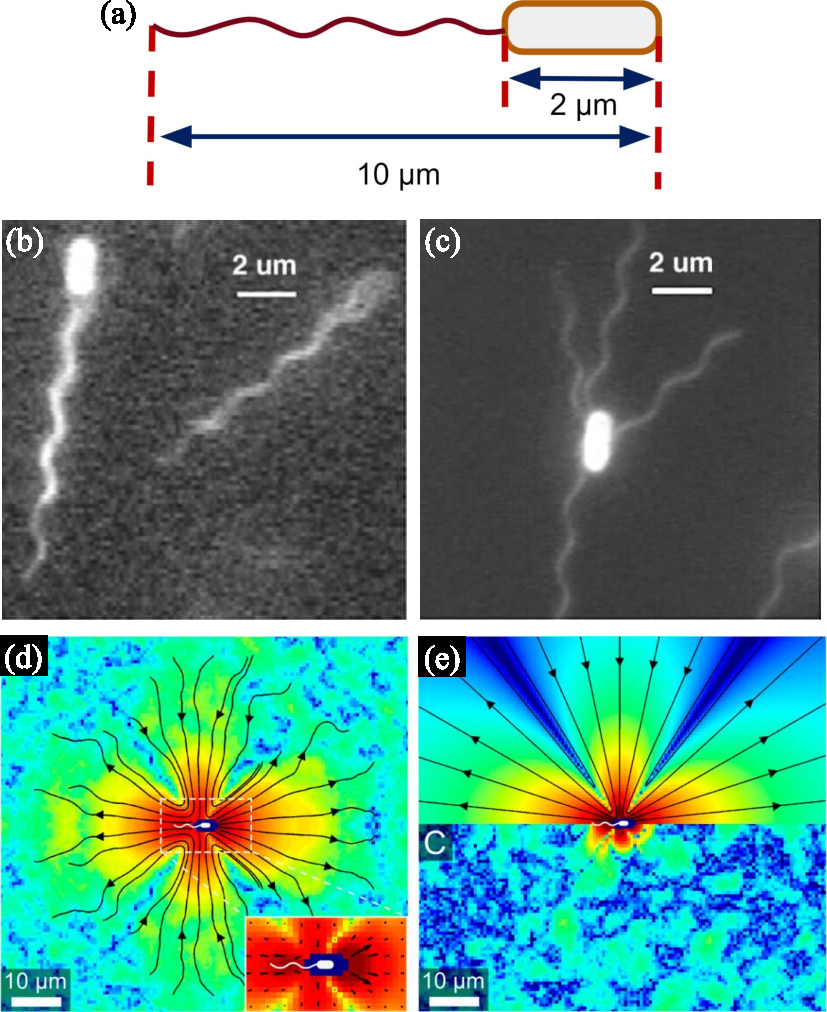
\includegraphics[height=5.5in]{Figs/2-Exp/1.pdf}
	%select pdftexify command to run jpg or pdf files
	\end{center}
	\caption[Model swimmer \textit{Escherichia coli} and its flow field]
	{
	\textbf{Model swimmer \textit{Escherichia coli} and its flow field.}
  (a) A schematic of a swimming \textit{E. coli} bacterium.
  (b) Fluorescence microscopic image of swimming \textit{E. coli} with bundled flagella.
  (c) Fluorescence microscopic image of tumbling \textit{E. coli} with unbundled flagella.
  (d) Flow field around a swimming \textit{E. coli}, measured with suspending microspheres.
  (e) Best-fit force dipole flow for the flow field shown in (d).
  Image sources:
  (b) and (c) are reprinted from Ref.~\cite{Turner2000} with permission from the American Society for Microbiology.
  (d) and (e) are reprinted from Ref.~\cite{Drescher2011} with permission from the NAS.
	}
	\label{fig:2-1}
\end{figure}

There are quite a few research groups over the world that are using \textit{E. coli} suspensions to study active fluids. To name a few, Yodh and Arratia at University of Pennsylvania, Wu at Cornell University, Poon at the University of Edinburgh and Clement at ESPCI all have published experimental works using \textit{E. coli} \cite{Chen2007, Patteson2016, Kasyap2014, Jepson2013, Mino2011}. Although the protocols of preparing motile \textit{E. coli} samples are similar across different groups' protocols, they have subtle differences from each other, which may be attributed to the specific strain of \textit{E. coli}, ingredients of media and specific instrument conditions. Schwarz-Linek et al. proposed a sample preparation protocol based on standard bioscience manuals \cite{Bonner2011}
and Berg's \textit{E. coli} protocol. If one wants to learn how to prepare motile \textit{E. coli} from scratch, it is recommended to follow the protocol in Ref.~\cite{Schwarz-Linek2016}.

When I joined the Cheng group at the University of Minnesota in 2015, before Ref.~\cite{Schwarz-Linek2016} was published, there was already a protocol in our lab that worked pretty well for us. I learned the protocol from previous lab members Yi Peng and Devranjan Samanta, and have made some modifications over the years  to optimize the motility and concentration of samples and to include the additional procedures for preparing light-powered \textit{E. coli}. Below I describe the protocol that works the best in Cheng lab.

\subsection{Background Information}
\begin{description}
  \item [Bacterial strains] We primarily work on two E. coli strains: \textit{AW804} and \textit{BW25113}. \textit{AW804} is light-sensitive. \textit{BW25113} is a wild type strain carrying a plasmid encoding green fluorescence protein, thus it is used when fluorescence / confocal microscopy is needed. Both strains have ampicillin resistance marker and thus require supplementing ampicillin to culturing media.
  \item [Antibiotics] Bacteria are ubiquitous in the environment and can easily  contaminate our bacterial culture. In order to ensure the fidelity of the culture, we add antibiotic resistance markers to the bacteria we want to grow and meanwhile add antibiotics to the medium. The antibiotics inhibit the growth of contaminating species and allow our desired bacteria to grow normally.
  \item [Medium] Various types of media (terrific broth, Luria broth, 2XYT and M9, etc.) are commonly used for bacterial culture. We use terrific broth. The recipe can be found in the protocol section.
\end{description}

\subsection{Protocol}
\label{sec:protocol}
\begin{enumerate}

  \item Prepare a 2-ml \textit{E. coli} overnight culture.

  \begin{enumerate}
    \item Prepare liquid terrific broth (TB). For example, to make 1 L TB, weigh out the following into a 1 L glass bottle:
    \begin{itemize}
      \item 23.6 g Yeast extract (Sigma-Aldrich)
      \item 11.8 g Tryptone plus (Sigma-Aldrich)
      \item 4 ml Glycerol (Thermo Fisher Scientific)
      \item Add dI water to 1 L
    \end{itemize}
    Loosely close the cap on the bottle (do NOT close all the way or the bottle may explode!) and then loosely cover the top of the bottle with autoclave tape (stick cap and bottle body together to avoid cap popping off). Autoclave and allow to cool to room temperature. Now screw on the top of the bottle and store the TB at room temperature.
    \item Using a sterile 10 ml pipette, transfer 2 ml TB to a sterile glass test tube.
    \item Using a sterile pipette, add 2 microliter (0.1\% v/v) antibiotic solution to the TB in test tube.
    \item Using a sterile pipette tip, pick a small chunk from our bacterial frozen stock (stored in the -80 °C freezer in 251) and carefully transfer the small chunk into the liquid TB + antibiotic.
    \item Loosely cover the culture with sterile cap that is not air tight.
    \item Incubate bacterial culture at 37 °C for 12-18 h in a shaking incubator.
    \item After incubation, check growth, which is characterized by a cloudy haze in the media. This is the overnight culture.
  \end{enumerate}

  \item Dilute overnight culture and harvest motile bacteria at mid-late log phase.
  \begin{enumerate}
    \item Using a sterile 10 ml pipette, transfer 3 ml TB to a sterile glass test tube.
    \item Using a sterile pipette, add 2 microliter (0.1\% v/v) antibiotic solution to the TB in test tube.
    \item Transfer 30 microliter (1\% v/v) overnight culture into the liquid TB + antibiotic.
    \item Incubate bacterial culture at 30 °C for 6-6.5 h in a shaking incubator.
    \item After incubation, check for growth, which is characterized by a cloudy haze in the media. This is the log phase bacteria.
  \end{enumerate}
  \item Centrifuge for better motility and higher concentration bacterial sample.
  \begin{enumerate}
    \item Prepare motility buffer (MB), the following recipe is from Ref.~\cite{Peng2016}.
    \begin{itemize}
      \item 0.01 M potassium phosphate (combine monobasic and dibasic solutions, Sigma-Aldrich)
      \item 10$^{-4}$ M EDTA (Sigma-Aldrich)
      \item 0.002\% weight fraction Tween 20 (Sigma-Aldrich)
      \item Adjust pH to 7.0
    \end{itemize}
    \item Take out the log phase bacteria from the shaking incubator, centrifuge for 5 min at 800 rcf.
    \item Discard the supernatant quickly and transfer the left-over liquid to a new centrifuge tube.
    \item Add 500-1000 ul MB (or water) to resuspend the bottom pellet (avoid bottom pellet) and centrifuge for a second time (5 min, 800 rcf).
    \item Discard the supernatant and let the tubes sit for two minutes. The remaining left-over liquid should be now filled with the active \textit{E. coli}. Take the left-over solution in another capsule and use it for experiments.
    \item To measure the concentration, transfer 10 microliter of the suspension into a 1 ml plastic cuvette (0.5 cm) and dilute 100 times (by adding 990 microliter water). Put the cuvette in the spectrophotometer (Eppendorf) and use the OD600 program. The resulting number times 100 will be the number density of your suspension in the unit of n$_0$ (8 x 10$^8$ cells/ml).
  \end{enumerate}
\end{enumerate}

\begin{figure}[ht]
	\begin{center}
	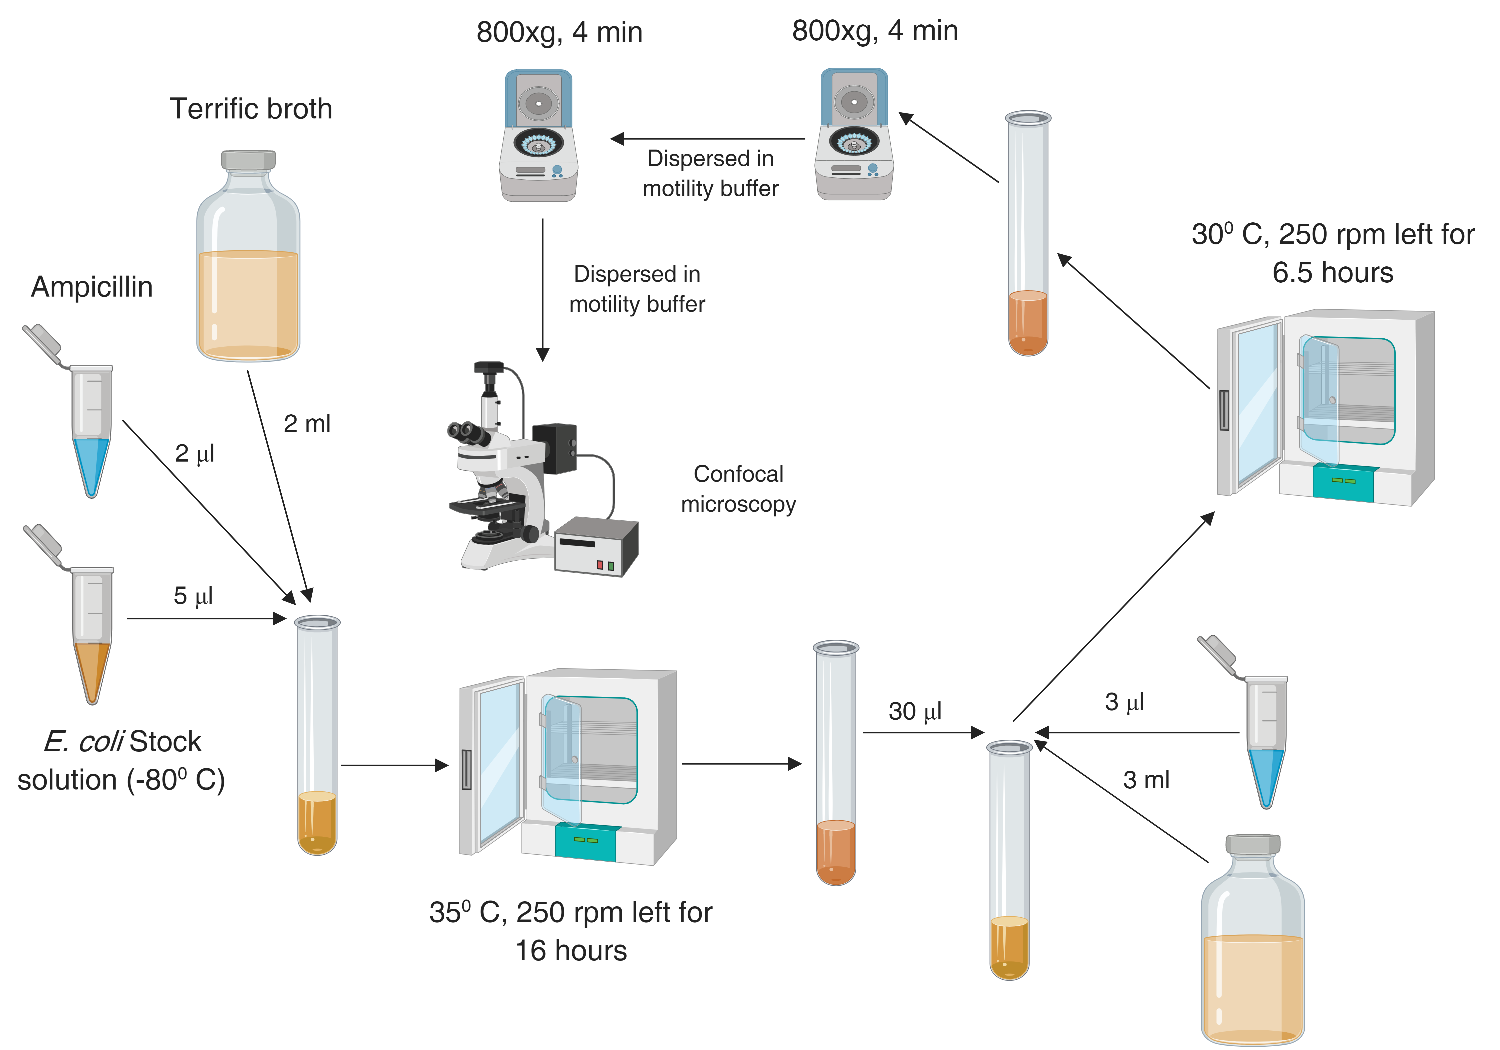
\includegraphics[width=5.5 in]{Figs/2-Exp/2.pdf}
	%select pdftexify command to run jpg or pdf files
	\end{center}
	\caption[Graphical motile \textit{E. coli} sample preparation protocol]
	{
	\textbf{Graphical motile \textit{E. coli} sample preparation protocol.}
	Image courtesy of Shashank Kamdar.
	}
	\label{fig:2-2}
\end{figure}





\section{Optical Microscopy}
\label{sec:optical-microscopy}

In this section, I will decribe how I overcome practical challenges when applying optical microscopy on bacterial suspensions. I want to note that the standard manuals are always the best reference for beginners who have just started to learn about a technique. In my case, the standard manuals are the Nikon inverted microscope Eclipse Ti-E Ti-E/B instructions \cite{NikonTiEManual}, OpenPIV official website \cite{OpenPIV-website, OpenPIV-paper} and trackpy official website \cite{trackpy-website}. Some related projects (listed in the websites mentioned) also provide valuable tutorials and ideas, for example the particle tracking routines in IDL by Crocker and Weeks \cite{IDL-tracking} and in Matlab by Blair and Dufresne \cite{Matlab-tracking}.

\begin{figure}[!htbp]
	\begin{center}
	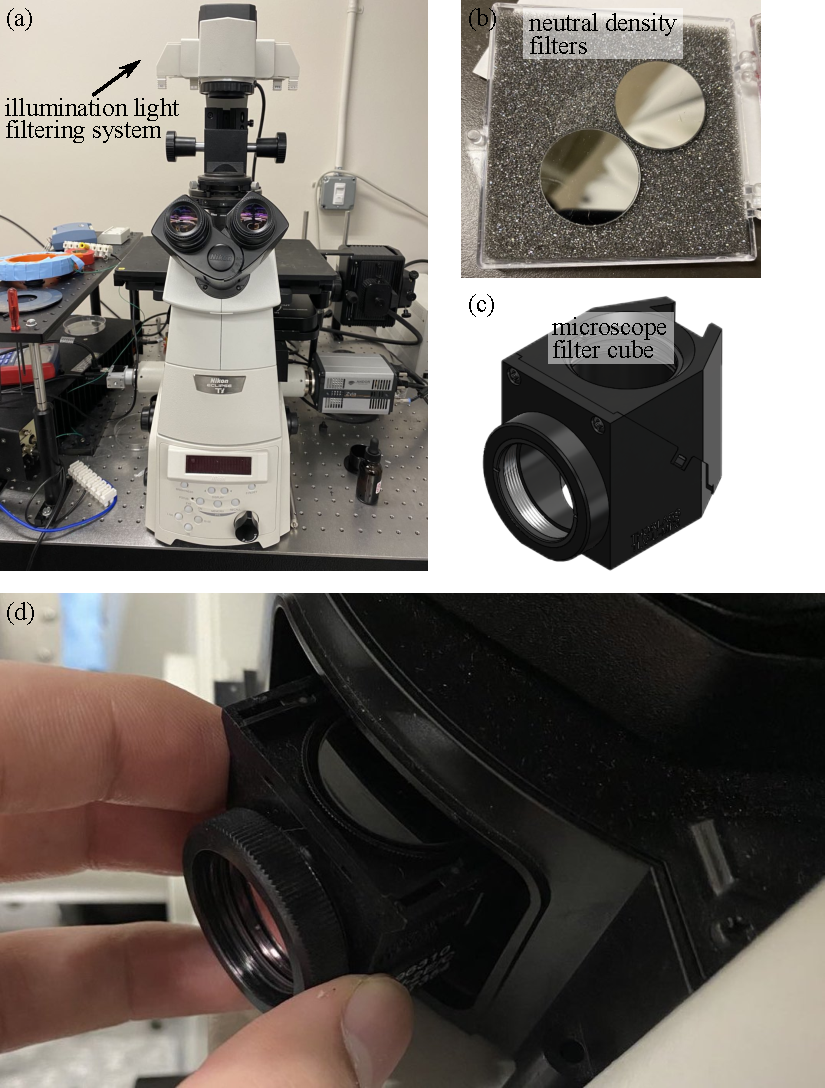
\includegraphics[width=5.5 in]{Figs/2-Exp/3.pdf}
	%select pdftexify command to run jpg or pdf files
	\end{center}
	\caption[Nikon Ti-E inverted microscope and its filters]
	{
	\textbf{Nikon Ti-E inverted microscope and its filters.}
	(a) Nikon Ti-E inverted microscope model.
	(b) Illumination light path filters.
	(c) Filter block under objective.
	(d) Adding additional ND filter under objective.
	}
	\label{fig:2-3}
\end{figure}

\subsection{Power \textit{E. coli} with Illumination Light}
In the studies of the giant number fluctuations and the emergence of active turbulence, I used a light-powered \textit{E. coli} mutant, which changes its swimming speed according to the amount of light it receives (details of the light-powered \textit{E. coli} mutant can be found in Sec.~\ref{light-controlled-E-coli-genetic-modification-culturing-and-trouble-shooting}).

I use the illumination light of the microscope as the power source of the bacteria, instead of using another light source, based on two considerations: 1) an additional light source shining on the sample will lead to additional unexpected light going into the objective, which often leads to bad image quality, 2) it is hard to construct a spatially uniform light, especially when it has to come in an angle not perpendicular to the specimen. Therefore, I use the illumination light of the microscope to power the \textit{E. coli}.

The light-powered \textit{E. coli} mutant requires quite a high light intensity to move fast enough. Such a high intensity cannot be achieved in the normal microscopy conditions, where four light filters are applied for different purposes. Fig.~\ref{fig:2-3}a and b show the Nikon Ti-E inverted microscope and the illumination light filtering system with the four light filters designated as ND, D, NCB and PFS. The functions of the filters are listed in Table.~\ref{table:2-1}:

\begin{table}[h]
	\centering
	\spacerows{1.2}
	\begin{tabular}{ | p{0.4in} | p{5in} |}
		\hline
		\textbf{ND} & Neutral density filter: adjust the brightness for normal microscopy or photomicroscopy \\
		\hline
		\textbf{D} & Diffusion filter: made of frosted glass and will diffuse light, used for equalizing the illumination \\
		\hline
		\textbf{NCB} & Neutral color balance: corrects the color temperature for mnormal microscopy or filming by daylight type color. Note: this filter is essential for optimal color reproducibility when taking color images, and it should be kept out of the optical path when filming in black and white. \\
		\hline
		\textbf{PFS} & Perfect focusing system: a hardware solution to combat axial focus fluctuations in real time during long-term imaging investigations. Note - this filter should be kept out if one does not intend to use the perfect focusing system.\\
		\hline
	\end{tabular}
	\caption[Filters in the illumination light path and their functions.]{Filters in the illumination light path and their functions.}
	\label{table:2-1}
\end{table}

Removing some of those filters can make the illumination light strong enough to power the bacteria. According to the functions of the filters, the only necessary filter is the diffusion filter, given that one is not doing color imaging and is not using perfect focusing system, as it is in my experiment. Fig.~\ref{fig:2-4}a shows an image taken without the diffusion filter (D). Without diffusing the illumination light, the resulting image is clearly inhomogeneous in a large range, with a bright center and a dark bottom area. By putting the diffusion filter in the illumination light path, one can make the illumination light much more uniform, as shown in Fig.~\ref{fig:2-4}b. All the other filters (ND, NCB, PFS) are effectively reducing the overall intensity. Putting in or out these filters only results in globally dimmer or brighter images, without changing the detailed patterns in the image. Thus, these three filters are optional in my experiment. Since powering the light-powered \textit{E. coli} requires a very high light intensity, only the diffusion filter should be kept in the illumination light path.

\begin{figure}[!]
	\begin{center}
	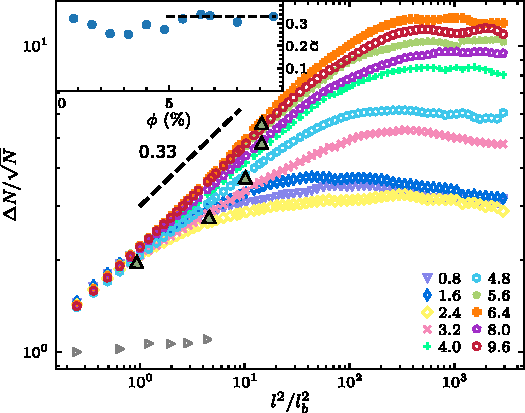
\includegraphics[width=5.5 in]{Figs/2-Exp/4.pdf}
	%select pdftexify command to run jpg or pdf files
	\end{center}
	\caption[Diffusion filter function illustration]
	{
	Image with (a) and without (b) the diffusion filter (D).
	}
	\label{fig:2-4}
\end{figure}

\subsection{Adding Filters to Avoid Overexposure}

While high enough light intensity is achieved to power the light-controlled bacteria, the light is so strong that the camera is overexposed and does not record any meaningful signal. In order to power the bacteria, the illumination light intensity cannot be reduced. The only way to avoid the overexposure is to add neutral density filters between the specimen and the camera, so that the light goes to the camera gets dimmer. Fig.~\ref{fig:2-3}c and d show how I placed the filters between the specimen and the camera. I took out one of the filter cube from the turret under the objective, which is originally used for fluorescence microscopy. Then I put a piece of neutral density filter on top of the cube and put the cube back to the turret. This additional filter allows for the imaging under strong illumination light.

\section{Image Analysis}
\label{sec:image-analysis}
With the fast developments of digital imaging, human are enabled to investigate many processes, ranging from astronomical object motions to microorganism behavior, in unprecedented detail \cite{Kalaidzidis2007}. While it is getting easier than ever to acquire large amount of images, a demand for automated image analysis has also become unprecedented \cite{Meijering2006, Jaqaman2008, Rohr2010}.

Particle tracking has been one of the most useful automated image analysis tools in the study of colloids and microorganisms. Over the last 20 years, it has developed significantly and many algorithms, toolkits and all-in-one softwares have been implemented and applied in a variety of image analysis tasks. Despite the abundance of particle tracking tools, no agreement has been made on which one in the vast collection of tools works best. Much effort has been devoted to answer this question by comparing the performance of different tools \cite{Kalaidzidis2007, Dorn2008, Meijering2009, Smal2010, Meijering2012,
Chenouard2014, Maska2014, Hilsenbeck2016}. In these studies, though different algorithms show different performance, no single algorithm outperforms all the others in all scenarios.

Particle tracking is generally composed of two steps: particle detection (spatial) and linking trajectories (temporal). For the detection step, based on the feature (generalized ``particle'') shape sought, different methods are used. For point features, a local maxima finding method is often used; for edge features, group labeling is often used; and for region features, region seeding is often used \cite{Dorn2008}.

\subsection{Anisotropic Particle Tracking}

A challenge I encountered when working on the diffusion project was the detecting of the ellipsoidal particles surrounded by moving microorganisms (bacteria and algae). A local maxima finding method was applied previously to detect the center of an ellipsoidal particle \cite{Han2006}. Combined with intensity fitting around the cneter in different directions, the orientation of the particle can also be obtained. The same method, however, does not work well for my image because of the presence of microorganisms, which give rise to many more local maxima in the image (a typical image is shown in Fig.~\ref{fig:2-5}a). To overcome this challenge, I adapted a thresholding and connected group labeling based method from Ref.~\cite{custom-feature-detection, Sauret2015, Cappello2015}. The method has the following steps:

\begin{figure}[!]
	\begin{center}
	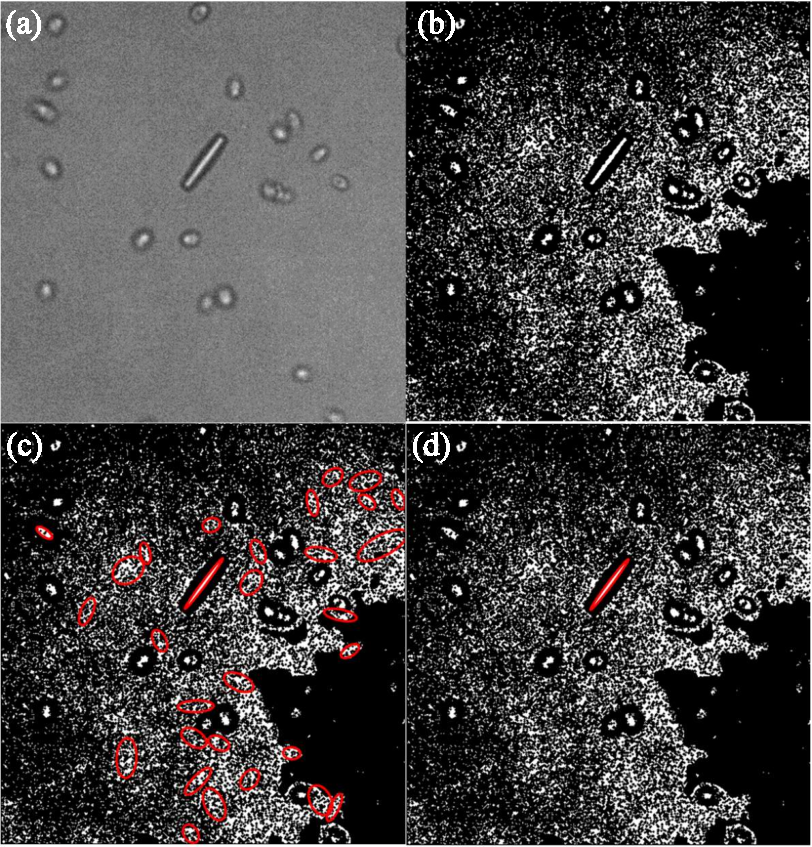
\includegraphics[width=5.5 in]{Figs/2-Exp/5.pdf}
	%select pdftexify command to run jpg or pdf files
	\end{center}
	\caption[Illustration of ellipsoidal particle detection by thresholding and group labeling]
	{
	\textbf{Illustration of ellipsoidal particle detection by thresholding and group labeling.}
	(a) The raw image: an ellipsoidal polystyrene particle surrounded by swimming algae in a suspension.
	(b) Binarized raw image.
	(c) Detection result of connected white regions.
	(d) Final result after appropriate filtering.
	}
	\label{fig:2-5}
\end{figure}

\begin{itemize}
	\item threshold the grayscale image (Fig.~\ref{fig:2-5}a) to a binary image (Fig.~\ref{fig:2-5}b)
	\item find connected white regions (\texttt{skimage.measure.label} in Python)
	\item find the best-fit ellipse of each white connected regions found in the last step, as indicated by the red ellipses in Fig.~\ref{fig:2-5}c (\texttt{skimage.measure.regionprops} in Python)
	\item filter the parameters of the ellipses with appropriate criteria, so that only the desired ellipse is found, as indicated by the red ellipse in Fig.~\ref{fig:2-5}d
\end{itemize}

Fig.~\ref{fig:2-5} only illustrates the essential idea of the method. When applying the method, some necessary image preprocessing, including linear, nonlinear and frequency filters need to be used to make sure the desired features stand out, and the undesired noises are suppressed. The preprocessing techniques have been reviewed in Ref.~\cite{Dorn2008, Rohr2010}. This method was used to obtain the trajectories of ellipsoidal particles in algal suspensions, which was then used to calculate the diffusivity for my first collaborative project, reported in Ref.~\cite{Yang2016}.

\subsection{Manual Particle Tracking Software: \textit{manTrack}}
Despite the great advances of particle tracking techniques, the accuracy suffers much from poor image quality and mutual touching of objects in images, especially when imaging dense suspensions of microorganisms \cite{Meijering2009}. A very challenging particle detecting task is manifested by a dense suspension of collectively moving bacteria, as shown in Fig.~\ref{fig:2-6}a. Despite the use of confocal microscopy, most bacteria are seen to be overlapping with others and are in very different shapes, making it impossible for existing tools to detect all the desired features. In a scenario like this, human eyes are the most powerful complementary tool to machines.

Manually marking the positions of particles is feasible when one image only contains one or several particles. When particle numbers get large, however, it is no longer feasible (a typical video I take contains hundreds of particles). I combined the automated tracking and the manual tracking together in order to take the advantages of both: fast and reliable, by implementing a manual tracking software \textit{manTrack} with graphical user interface (GUI). The workflow for using \textit{manTrack} is:

\begin{itemize}
	\item Use an automated method to do a preliminary particle tracking (or detection).
	\item Load the preliminary automated detection result into \textit{manTrack}. The result will be displayed in \textit{manTrack} GUI as elliptical contours, as shown in Fig.~\ref{fig:2-6}b.
	\item When ``delete mode'' is enabled, one can delete one entry from the result by clicking on the elliptical contour. In Fig.~\ref{fig:2-6}c, the entry at the tip of the red arrow has been deleted.
	\item When ``track mode'' is enabled, one can add an entry to the current result by drawing an ellipse in the image, as shown by the black contour in Fig.~\ref{fig:2-6}d.
\end{itemize}

\textit{manTrack} provides a user friendly GUI for efficient modification of preliminary automated particle detection results. The combination of machine automated detection and human eye detection makes possible good accuracy and an acceptable execution speed. This software was used for analyzing the orientation of bacteria in active turbulence (Chap.~\ref{the-emergence-of-active-turbulence}).

Several new tools have been developed in recent years, such as \textit{TrackMate} and \textit{tTt} \cite{Tinevez2017, Hilsenbeck2016}. The fast growth of technologies in other fields, especially artificial intelligence, has stimulate the development of new tracking techniques \cite{Newby2018, Moen2019}.

\begin{figure}[!ht]
	\begin{center}
	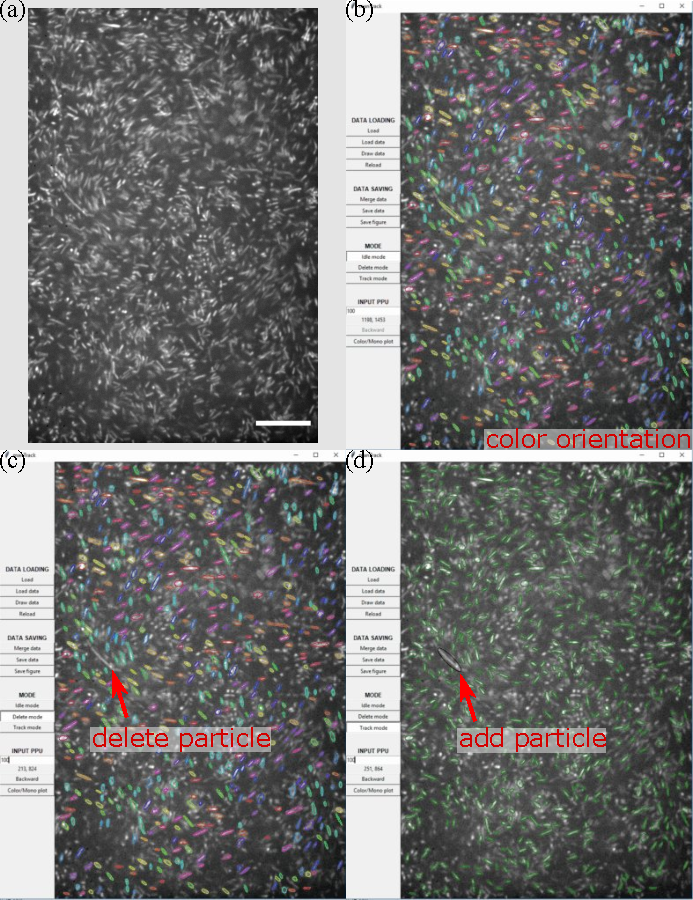
\includegraphics[height=5.5 in]{Figs/2-Exp/6.pdf}
	%select pdftexify command to run jpg or pdf files
	\end{center}
	\caption[A challenging particle detection task and the manual tracking software]
	{
	\textbf{A challenging particle detection task and the manual tracking software.}
	(a) Confocal microscopy image of \textit{E. coli} collective motion ($\phi=6.4\%$).
	(b)-(d) Snapshots of the manTrack software, demonstrating color-coded orientation, manual deleting and manual adding.
	}
	\label{fig:2-6}
\end{figure}

\subsection{Particle Image Velocimetry }
Particle image velocimetry (PIV) is a method of visualizing flow using based on images. It is used to obtain instantaneous fluid velocity fields by comparing positions of tracer particles in the fluids in consecutive image frames. The tracer particles are assumed to follow the flow faithfully all the time, and this assumption is in general valid when when particle size is small. The degree of how faithful the tracers follow the flow is quantified by Stokes number, which compares the intrinsic relaxation time scale and the characteristic time scale of the flow.

\begin{figure}[!ht]
	\begin{center}
	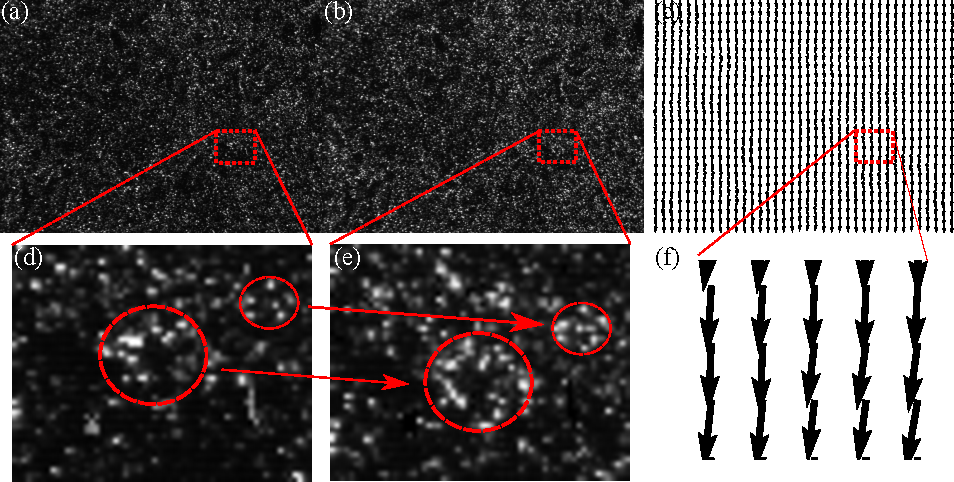
\includegraphics[width=5.5in]{Figs/2-Exp/PIV.pdf}
	%select pdftexify command to run jpg or pdf files
	\end{center}
	\caption[PIV working principle illustration]
	{
	\textbf{PIV working principle illustration.}
	(a) and (b) are images of fluid flows seeded with tracer particles. (c) is the instantaneous velocity field in (a) and (b), obtained from PIV. (d) and (e) are zoom-in's of the two images in a small window. Circles indicates similar image features in (d) and (e). (f) is a zoom-in of velocity field.
	}
	\label{fig:PIV}
\end{figure}


The comparison between two image frames is done by dividing the images in to small interrogation windows and computing the correlations of the two images in these windows, which essentially looks for the similar features between the two images. This procedure is illustrated in Fig.~\ref{fig:PIV}. Fig.~\ref{fig:PIV}a and b are two example images and Fig.~\ref{fig:PIV}c shows the instantaneous flow field obtained from PIV analysis. The result suggests that there is a global flow going to the bottom of the images. Though it is not so obvious in the original images, if we zoom in to a small region, as shown in Fig.~\ref{fig:PIV}d and e, the similar features (indicated by red circles) get obvious and we therefore expect the flow going to the bottom of the images, as shown in Fig.~\ref{fig:PIV}f.

Invented in the 1970s, PIV has been developed into a mature flow velocimetry technique today. Several implementations of the algorithm are present in different programming frameworks, such as Matlab, Mathametica and Python. In this work, we use an open source PIV toolkit \textit{OpenPIV} written in Python, which is maintained by Liberzon and co-workers \cite{OpenPIV-website, OpenPIV-paper}.

\subsection{Spatial and Temporal Correlation Functions}

Spatial (temporal) correlation functions describe how variables, such as velocity and density, at different positions (time) are related. It measures the order in a system. These functions are used in the study of giant number fluctuations to measure the characteristic length and time in bacterial suspensions of different volume fractions (Chap.~\ref{giant-number-fluctuations-in-3-dimensional-space}).

The correlation functions have been defined clearly in statistical mechannics and mathematics. For example, the spatial correlation function of number density $n(\bm{r})$, $C_n(\bm{R})$ is
\begin{equation}
	\label{eq:correlation-function}
	C_n(\bm{R}) = \frac{\langle n(\bm{r})\cdot n(\bm{r}+\bm{R}) \rangle - \langle n(\bm{r})\rangle \langle n(\bm{r}+\bm{R})\rangle}{\sigma_{n(\bm{r})}^2}
\end{equation}
%
where $\langle A \rangle$ denotes the spatial average of $A$, and $\sigma_A$ denotes the standard deviation of $A$.

Although the definition is clear, the programming implementation can be quite different in efficiency. When implementing these correlation functions, I learned an important trick---code vectorization---which can speed up the computation of correlation functions up to 50 times. The enhancement of performance gets more pronounced when the input data is larger. Therefore, I would like to document this knowledge here.


\begin{figure}[!ht]
	\begin{center}
	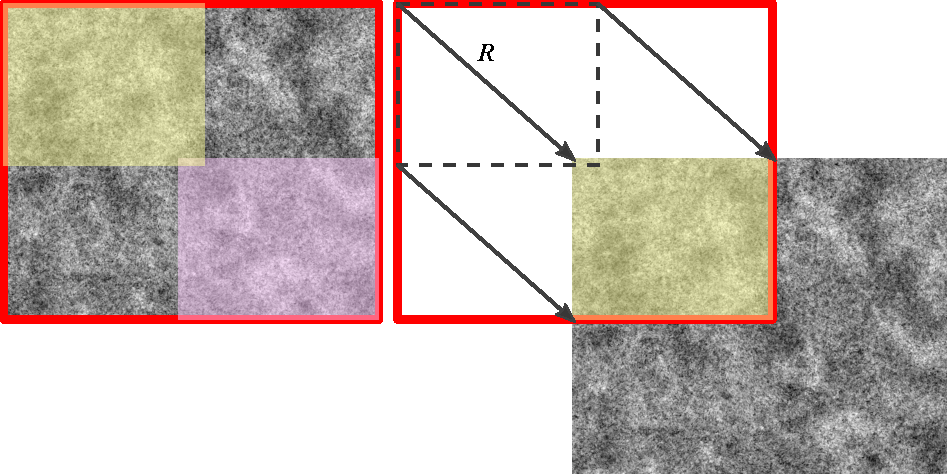
\includegraphics[width=5.5in]{Figs/2-Exp/vectorization.pdf}
	%select pdftexify command to run jpg or pdf files
	\end{center}
	\caption[Code vectorization illustration]
	{
	\textbf{Code vectorization illustration.}
	The correlation function at a certain distance $\bm{R}$, $C(\bm{R})$ can be calculated without using a \texttt{for} loop. Two subspaces are identified from the whole space, as indicated by purple and yellow shaded regions, which are $\bm{R}$ away from each other. $C(\bm{R})$ can be calculated by taking the product of these two subspaces and then taking the mean of this product.
	}
	\label{fig:vectorization}
\end{figure}


The calculation of the correlation function in Eq.~\ref{eq:correlation-function} requires going over the whole space twice: for each point $\bm{r}$ in the space, all possible distance $\bm{R}$ needs to be examined. In two dimensional space, this procedure leads to four \texttt{for} loops. The basic idea of code vectorization is to avoid the extensive use of \texttt{for} loops. In this specific case, for every possible distance $\bm{R}$, the correlation can be calculated without using a \texttt{for} loop, by directly calculating the product of two subspaces and the taking average, as illustrated in Fig.~\ref{fig:vectorization}. Two subspaces are identified from the whole space, which are $\bm{R}$ away from each other, as indicated by purple and yellow shaded regions. Note that matrix product calculation is well optimized in almost all programming languages and is much faster than looping over every element in a matrix. Using this trick, only two \texttt{for} loops are necessary, which go over all possible distances $\bm{R}$. The Python implementations of spatial and temporal correlation functions, as well as a speed comparison between non-vectorized and vectorized programs, can be found in Appendix.~\ref{sec:A-vectorization}.

\subsection{Energy Spectrum Calculation}
As discussed in Sec.~\ref{sec:intro-GNF}, energy spectra have been widely used for studying the flow structure of classic turbulent flows, by revealing the kinetic energy disctribution over different length scales. Here, we show the details in the method of calculating energy spectra of the flow in bacterial suspensions at various volume fractions, using the velocity fields obtained from PIV analysis. This calculation will be used in Chap.~\ref{the-emergence-of-active-turbulence} and Chap.~\ref{giant-number-fluctuations-in-3-dimensional-space}.

The energy spectra of bacterial suspensions are calculated as the following
%
\begin{equation}
E(k_x, k_y) = \frac{\langle u_k(k_x, k_y)u^*_k(k_x, k_y)+v_k(k_x, k_y)v_k^*(k_x, k_y)\rangle}{2A}
\end{equation}
%
where $E$ is the energy density in $k$ space, $u_k$ and $v_k$ are $k$ space velocity fields, $A$ is the real space area of the system and $^*$ denotes the complex conjugate. The $\langle\cdot\rangle$ denotes an average over multiple images from different times.

The fourier transform of real space velocity $u_k$ and $v_k$ are computed as the following:
\begin{itemize}
  \item apply the built-in Fast Fourier Transform (FFT) function of Python \texttt{numpy.fft} package to the discrete velocity field $v(x, y)$ (from PIV) to get $V_k(k_x, k_y)$
  \item since the FFT is defined as
    $$
    V_k=\sum^{n-1}_{m=0}v_m\exp(-2\pi i \frac{mk}{n})
    $$
    missing the $dx$ counterpart in the continuous Fourier transform, we additionally multiply $d_{step}^2$ to $V_k(k_x, k_y)$ to get the wavenumber domain velocity $v_k(k_x, k_y)$
  \item the wavenumber field $k$ corresponding to $v_k(k_x, k_y)$ is obtained by applying the \texttt{numpy.fft.fftfreq} function. Since the definition of FFT introduces a prefactor $2\pi$ to the wavenumber, an additional $2\pi$ is also multiplied to $k$
\end{itemize}

The calculation described above is implemented in a Python code, which can be found in Appendix.\ref{sec:A-energy-spectra}.

\subsection{Other Image Analysis Tools}

\begin{itemize}
	\item Particle tracking based on image cross-correlation (Appendix.\ref{sec:A-cross-correlation-tracking-method})
	\item Orientation tracking based on Fast Fourier Transform (FFT) (Appendix.\ref{sec:A-fourier-transform-based-orientation-analysis})
	\item Density fluctuation calculations (Appendix.\ref{sec:A-df-calculation})
\end{itemize}


\section{Micro-fabrication and Microfluidic Viscometer}
\label{micro-fabrication-and-microfluidics}

\subsection{Micro-fabrication}

We used a standard micro-fabrication technique, soft lithography, to produce the microfluidic viscometer we used in the rheology project (Chap.~\ref{rheology-of-bacterial-suspensions-under-confinement}) \cite{Qin2010}. Such a fabrication usually involves the following steps: experimental design, pattern design, mask fabrication, master fabrication and elastomeric stamp fabrication.
After deciding on using the Y-shaped channel viscometer (Fig.~\ref{fig:experiment-microfluidics}a) \cite{Gachelin2013}, I did the pattern design and the staff at Minnesota Nano Center (MNC) had the mask fabricated for me. With the mask, I fabricated the masters of the Y-shaped channel viscometer for various channel heights using the MNC facilities. Then the masters were used for fabricating elastomeric stamps, using Sylgard 184 Silicone Elastomer Kit (Dow Inc.).

To produce masters for the various channel heights, different photoresists need to be used. I chose the SU-8 3000 series photoresists due to their good adhesion property and reduced coating stress, as well as their ready avaliability in the MNC labs. SU-8 3025 was used for channel heights from 25 to 50 $\mu$m. SU-8 3050 was used for channel heights from 50 to 128 $\mu$m. Following the procedures described in the photoresist manual, which includes substrate preparation, spin coating, soft bake, exposure, post exposure bake and develop, a photoresist patterned silicon wafer can be produced (Fig.~\ref{fig:experiment-microfluidics}b).

\begin{figure}[!ht]
	\begin{center}
	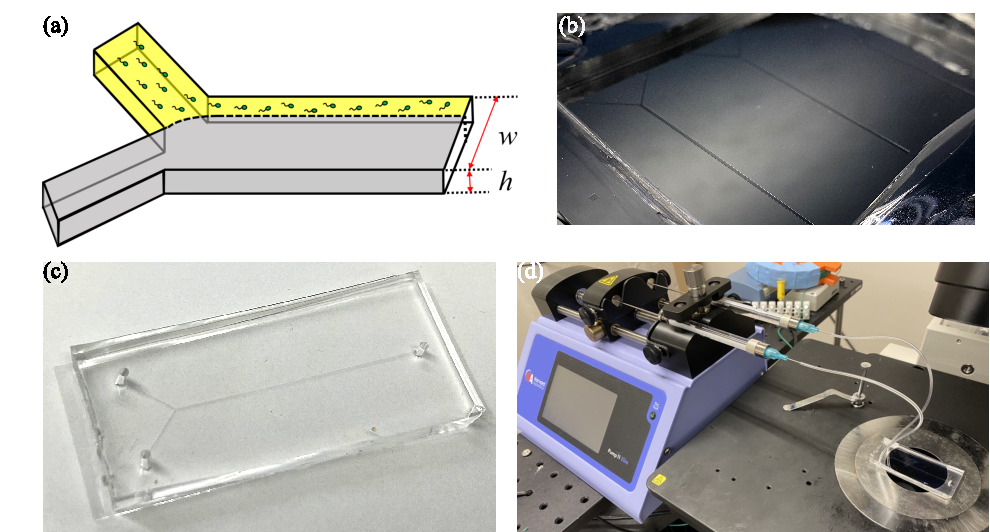
\includegraphics[width=5.5 in]{Figs/2-Exp/7.pdf}
	%select pdftexify command to run jpg or pdf files
	\end{center}
	\caption[Microfluidic viscometer fabrication and setup.]
	{
	\textbf{Microfluidic viscometer fabrication and setup.}
	(a) A sketch of the Y-shaped channel microfluidic viscometer.
	(b) Master mold of the channel.
	(c) PDMS Y-shaped channel microfluidic viscometer.
	(d) Viscometer connected to a syringe pump by plastic tubes, placed on Nikon inverted microscope specimen stage.
	}
	\label{fig:experiment-microfluidics}
\end{figure}

The elastomeric stamp is fabricated by pouring the Sylgard 184 Silicone Elastomer Kit, which contains a base and a crosslinker in a volume ratio 10:1, onto the photoresist masters. After curing for 3 hours at 70 °C, the pattern of the master mold was perfectly replicated on the solidified elastomer. Finally, a piece of coverslip was stuck on the patterned side of the elastomer by plasma cleaning the surfaces of both. The microfluidic channel is shown in Fig.~\ref{fig:experiment-microfluidics}c. The length and width of the two arms are 1 cm and 300 $\mu$m, respectively. The length and width of the main channel are 4 cm and 600 $\mu$m, respectively. The height of the channel $h$ ranges from 25 $\mu$m to 128 $\mu$m. Two cylindrical holes were punched at the ends of the two arms so that fluids can be pumped in.

\subsection{Microfluidic Viscometer}


To use the elastomeric stamp as a microfluidic viscometer, we connected it with a precision syringe pump (Harvard Apparatus, Elite 11) through elastic tubes, as shown in Fig.~\ref{fig:experiment-microfluidics}. The two syringes contained two different fluids: one was the bacterial suspension with viscosity to be measured, and the other was a reference fluid with known viscosity, typically water. The two fluids were pumped into the viscometer at the same volumetric flow rate $Q$.

The working principle of the viscometer is that thicker fluids flow slower than thinner ones. More formally, if we examine a fluid with viscosity $\eta$, driven by a pressure gradient $\diff p/\diff x$ to flow in the $x$-direction between two parallel no-slip boundaries at $z=\pm h/2$, as shown in Fig.~\ref{fig:experiment-microfluidics}a. At low Reynolds number limit, the flow rate regime of interest, the flow is governed by Navier-Stokes equation
\begin{equation}
	0 = -\frac{\diff P}{\diff x} + \eta \frac{\diff^2 u_x}{\diff z^2}
\end{equation}
The resulting flow is parabolic in $x$-$z$ plane and is approximately constant in $y$-direction, and can be described by Eq.~\ref{eq:parabolic-flow}
\begin{equation}
	\label{eq:parabolic-flow}
	u_x(z) = \frac{1}{2\eta}\frac{\diff P}{\diff x} (\frac{y^2}{h^2}-\frac{1}{4})
\end{equation}
For two different fluids with viscosities $\eta_1$ and $\eta_2$, the mean flow velocity in $x$-direction $\langle u_1 \rangle$ and $\langle u_2 \rangle$ are related to each other by
\begin{equation}
	\label{eq:velocity-viscosity}
	\frac{\langle u_1 \rangle}{\langle u_2 \rangle} = \frac{\eta_2}{\eta_1}
\end{equation}
noting that the flow rate $Q=\langle u \rangle dh$, where $d$ is the width ($y$-direction) of the flow, we can substitue the velocities $\langle u_1 \rangle$ and $\langle u_2 \rangle$ in Eq.~\ref{eq:velocity-viscosity} to get
\begin{equation}
	\label{eq:working-principle}
	\frac{d_1}{d_2} = \frac{\eta_1}{\eta_2}
\end{equation}
Eq.~\ref{eq:working-principle} is the working equation of the microfluidic viscometer. By imaging and measuring the width $d_1$ and $d_2$ of the two fluids in the channel, and combining the known viscosity of the reference fluid $\eta_2$, we can measure $\eta_1$.


\section{Light-controlled \textit{E. coli}: Genetic Modification and Culturing}
\label{light-controlled-E-coli-genetic-modification-culturing-and-trouble-shooting}
Controlling the swimming speed of swimmers can enormously expand the capability of experimental active fluid investigations. Our lab used to exploit a ``negative phototaxis'' property of a mutant \textit{E. coli} strain to control its swimming speed. The mutant strain carries a \textit{hemH} gene knockout, so that it accumulates protoporhyrin IX. When exposed to blue light, protoporhyrin IX catalyzes the production of H$_2$O$_2$, which causes the ``negative chemotaxis'' tumbling response of the \textit{E. coli} mutant \cite{Yang1995}. Although this mutant strain enables us to reduce the swimming speed, the recovery of swimming speed remains challenging due to the excessive production and accumulation of toxic H$_2$O$_2$. Hence, some important experiments, such as the study of the onset of active turbulence, which will be detailed in Chap.~\ref{the-emergence-of-active-turbulence}, cannot be done with this strain.

An alternative mechanism that can be exploited to control bacterial swimming speed is to introduce a light-driven proton pump protein, proteorhodopsin (PR), to \textit{E. coli}. PR protein has been found in marine micro-organisms \cite{Beja2000, DelaTorre2003}, and has recently been successfully expressed in \textit{E. coli} \cite{Walter2007}. In contrast to the \textit{hemH} knockout mutant, PR is much less harmful and provides better recovery of swimming speed. Therefore, I transformed the wildtype \textit{E. coli} K-12 strain BW25113 (Ref.~\cite{Datsenko2000}) with a plasmid pZE-PR containing the gene that encoded the PR protein. The sequence of the PR gene was found in Ref.~\cite{DelaTorre2003} and was sythesized by Eurofins Scientific.
The plasmid was constructed by the standard protocol consisting of PCR, enzymatic digestion and ligation. The PCR was carried out with Phusion High-Fidelity DNA polymerase (New England BioLabs) according to the manufacturer's instructions. Both the plasmid vector pZE and the PR gene were digested with Acc651-Xba1, and were subsequently ligated. XL10-Gold \textit{E. coli} strain was used for cloning the plasmid. Finally, the wildtype strain BW25113 was transformed with the plasmid by electro-poration and the light-controlled \textit{E. coli} mutant strain was constructed. The details of bacterial strains, plasmids and primers used in this work are listed in Table.~\ref{table:genetics}.

\begin{table}[!ht]
	\centering
	\spacerows{1.2}
	\begin{tabular}{lcl}
		% \toprule
		% Name                & Relevant genotype or sequence     & Reference         \\
		% \midrule
		% \textit{Strains}   & & \\
		% BW25113 & $rrnB_{T14}$ $\Delta lacZ_{WJ16}hsdR514$ $\Delta araBAD_{AH33}$ $\Delta rhaBAD_{LD78}$ &  \cite{Datsenko2000} \\
		% XL10-Gold     & Tet$^R$ $\Delta(mcrA)183$ $\Delta(mcrCB$-$hsaSMR$-$mrr)173$ $endAlsupE44$ $thi$-$l$ $recAl$ &  Stratagene     \\
		% \textit{Plasmids} & & \\
		% pZE-PR     & ColE1 origin, Amp$^R$, P$_LlacO_1$: $PR$ &  This work     \\
		% \textit{Primers} & & \\
		% PR-Acc651-F       & CCCGGGGGTACCATGAAGTTGTTGTTGATCTTGGGAT        &      \\
	  % PR-Xba1-R         & CCCGGGTCTAGATTATGCGTTCGATGACTCTTTCACG        &     \\
		% \bottomrule
		\hline
		name  &  Relevant genotype or sequence  &  Reference  \\
		\hline
		\emph{Strains}  &  &  \\
	  \multirow{2}{1em}{BW25113}  &  $rrnB_{T14}$ $\Delta lacZ_{WJ16}hsdR514$ $\Delta$  &  \multirow{2}{1em}{\cite{Datsenko2000}}  \\
															  &  $araBAD_{AH33}$ $\Delta rhaBAD_{LD78}$             &                          \\

		\multirow{2}{5em}{XL10-Gold}  &  Tet$^R$ $\Delta(mcrA)183$ $\Delta(mcrCB$-$hsaSMR$  &  \multirow{2}{1em}{\emph{Stratagene}}  \\
															    & -$mrr)173endAlsupE44$ $thi$-$l$ $recAl$             &                                 \\
	  \emph{Plasmids}  &  &  \\
	  pZE-PR  &  ColE1 origin, Amp$^R$, P$_LlacO_1$: $PR$  &  This work  \\
	  \textit{Primers} & & \\
 		\multirow{2}{8em}{PR-Acc651-F}  &  CCCGGGGGTACCATGAAGTT  &  \\
																	  &  GTTGTTGATCTTGGGAT     &  \\

	  \multirow{2}{8em}{PR-Xba1-R}   &  CCCGGGTCTAGATTATGCG  &  \\
																   &  TTCGATGACTCTTTCACG   &  \\
		\hline
	\end{tabular}
	\caption[Strains, plasmids and primers]
	{Strains, plasmids and primers.}
	\label{table:genetics}
\end{table}

The chromophore retinal molecule is essential for the PR protein to function as a proton pump. The retinal is isomerized upon illumination, and in this way it drives the proton transportation across cell membrane \cite{Subramaniam2000}. \textit{E. coli} does not synthesize such molecules. In order to activate the function of PR in \textit{E. coli}, we need to supplement the culturing media of \textit{E. coli} with retinal, in the form of ethanol solution of all-trans-retinal (Sigma-Aldrich). Typically, a 10 mM all-trans-retinal solution is prepared as a stock solution. When supplementing the culturing media, 1/1000 volume of retinal solution is used to achieve a final concentration 10 $\mu$M. To trigger the expression of PR gene under a P$_Llac$ operon, we also need to supplement the culturing media with another chemical Isopropyl $\beta$-D-1-thiogalactopyranoside (IPTG, Sigma-Aldrich) at a final concentration 1 mM. Therefore, when culturing the light-controlled \textit{E. coli}, an additional step needs to be added to the standard protocol (described in Sec.~\ref{sec:protocol}) between step 2(c) and 2(d). Typically, 3 hours after step 2(c), retinal and IPTG are supplemented to the culturing media.
